\documentclass{ps}

\ps{10}
\date{2019}
\author{}
\coauthor{}

\begin{document}
\begin{enumerate}
\item Modify the multicycle-cycle ARM processor to implement the BL
  instruction.  Mark up copies of the controller, main decoder FSM,
  ALU decoder, and datapath (attached) {\figurebelow} to handle the
  new instruction as simply as possible.  Name any control signals you
  need to add.
  \begin{center}
    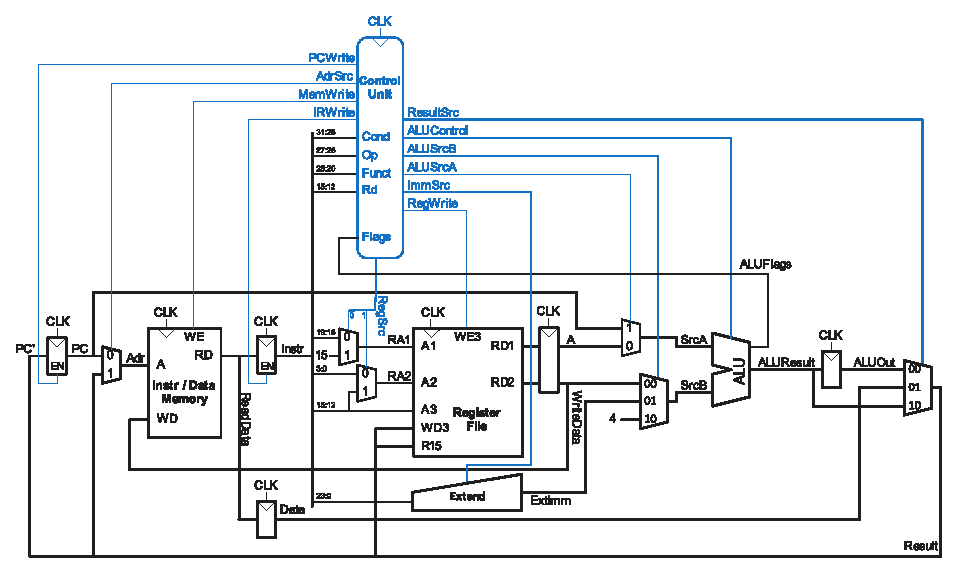
\includegraphics[width=\linewidth]
    {figures/ddca-complete-multicycle-processor.eps}
  \end{center}

  \begin{solution}
  \end{solution}

\item Goliath Corp claims to have a patent on a three-ported register
  file.  Rather than fighting Goliath in Court, you offer to design a
  newe register file with only two ports.  Port 1 can be read or
  written, and port 2 is read-only.  Redesign the multicycle datapath
  and controller (attached) {\figurebelow} to use your new register
  file.
  \begin{center}
    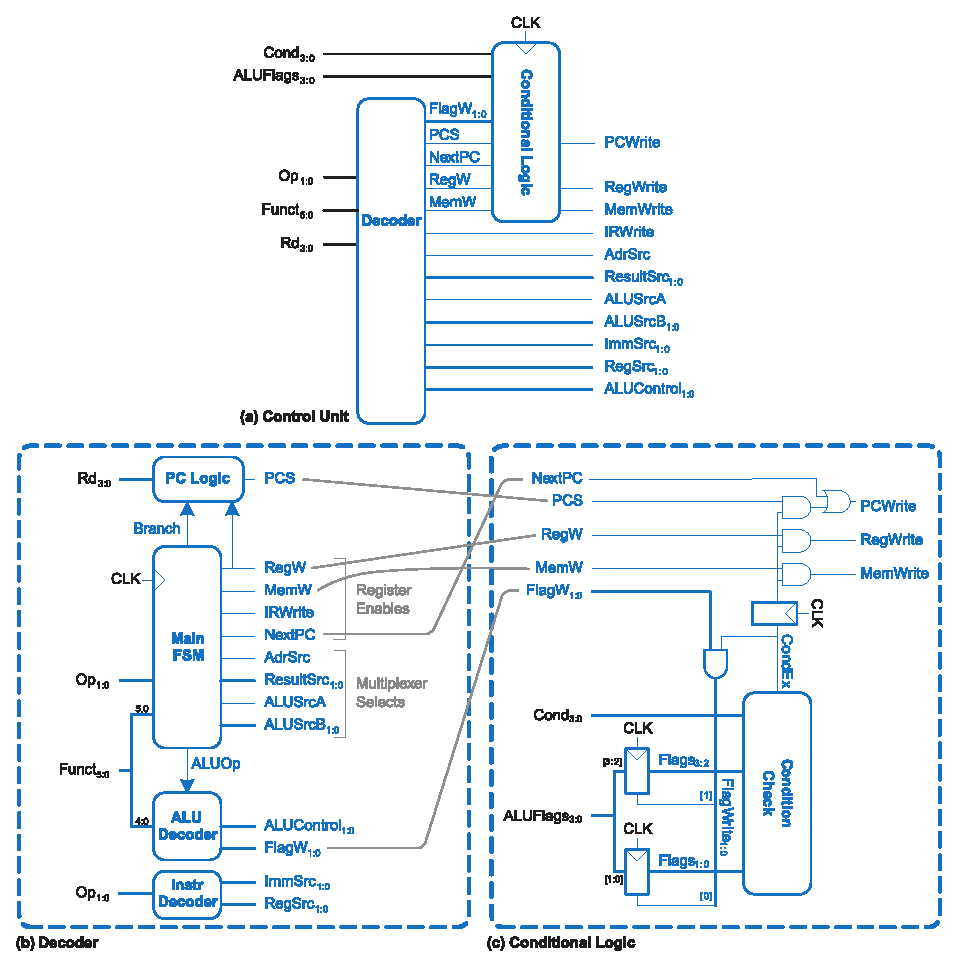
\includegraphics[width=\linewidth]
    {figures/ddca-multicycle-control-unit.eps}
  \end{center}

  \begin{solution}
  \end{solution}

\item How long would your processor from the previous question take to
  execute the 10-billion instruction program from Example 7.6?  Assume
  your new register file has \SI{30}{\percent} lower clk-to-Q and
  setup time because it has fewer ports but ordinary registers and
  other blocks have delay unchanges.

  \begin{solution}
  \end{solution}

\item Do Exercise 7.28 from the textbook.

  \begin{description}
  \item[7.28] The pipelined ARM processor is running the following
    code snippet.  Which registers are being written, and which are
    being read on the fifth cycle?  Recall that the pipelined ARM
    processor has a Hazard Unit.

    \inputminted{text}{code/ddca-7.28.arm}

    \begin{solution}
    \end{solution}
  \end{description}

\item Do Exercise 7.30 from the textbook.

  \begin{description}
  \item[7.30] Using a diagram similar to Figure 7.53 \figurebelow,
    show the forwarding and stalls needed to execute the following
    instructions on the pipelined ARM processor.

    \inputminted{text}{code/ddca-7.30.arm}

    \begin{solution}
    \end{solution}
  \end{description}

\item Impact on Society: Write a thoughtful paragraph describing a
  concrete example of how the skills you have developed in E85 may be
  applicable to another field of engineering in which you are
  interested in practicing.

  \begin{solution}
  \end{solution}
\end{enumerate}

How long did you spend on this problem set?  This will not count
toward your grade but will help calibrate the workload.
\begin{solution}
\end{solution}
\end{document}